\chapter{Renormalization and Envelopes}
The idea is that renormalization may possibly subsume/unify everything that has been done in this course: WKB, BL, multiple scales etc.! The Renormalization Group approach to singularly perturbed PDEs and ODEs was pioneered by Chen, Goldenfeld and Oono. But in this lecture we will focus on a \href{https://arxiv.org/abs/hep-th/9505166}{paper} by T. Kunihiro\footnote{``A Geometrical Formulation of the Renormalization Group Method for Global Analysis'', Prog. Theo. Phys. {\bf 94} (1995) 503.}: \\

 {\small {\bf Abstract. }{On the basis of classical theory of envelopes, we formulate the Renormalization Group (RG) method of global analysis, recently proposed by Goldenfeld et al. It is clarified in a generic way why the RG equation improves the global nature of function obtained in the perturbation theory. }}


\paragraph{Example 1:} Find the envelope of the family of straight lines which are of unit length between their $x$ and $y$ intercepts (like a ladder sliding down a wall). This looks like there is a bounding curve ``envelope'' such that each tangent line (ladder equation at some $t$) is tangent to this envelope. 
\begin{figure}[!h]
	\centering
	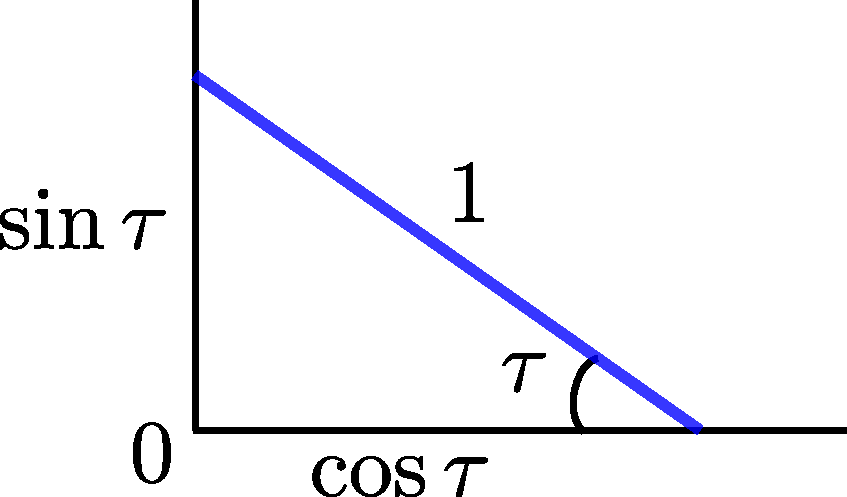
\includegraphics[width=0.33\textwidth]{./plots/pdf/renormalization-ladder.pdf}
	\caption{Ladder of unit length.}
	\label{fig:wk27-ladder}
\end{figure}\\
Noting that the slope $m$ and intercept $c$ are
\begin{gather*}
	m = -\frac{\sin \tau}{\cos \tau} \qquad c = \sin \tau
\end{gather*}
The equation of the line in terms of the parameter $\tau$ reads
\begin{gather*}
	\frac{y}{\sin \tau} + \frac{x}{\cos \tau}  = 1
\end{gather*}
We rewrite the family as $F(x,y,\tau)=0$ where
\begin{gather*}
	F(x,y,\tau) = y \cos \tau + x \sin \tau - \sin\tau \cos\tau
\end{gather*}
The envelope condition is 
\begin{gather*}
	F=0, \qquad \frac{\pd F}{\pd \tau} = 0
\end{gather*}
This yields 
\begin{gather*}
	-y \sin \tau + x \cos \tau + (\sin^2 \tau - \cos^2\tau  ) = 0 \\
	y \cos \tau + x \sin \tau - \sin\tau \cos\tau = 0
\end{gather*}
Multiplying the first equation with $\cos \tau$ and the second with $\sin \tau$ and adding, we derive
\begin{gather*}
	x = \cos^3 \tau \qquad y = \sin^3 \tau
\end{gather*}
The envelope equation is finally
\begin{gather*}
	x^{2/3} + y^{2/3} = 1
\end{gather*}
{\color{red} To do:}
\begin{itemize}
	\item Derive envelope equation and add to appendix
	\item plot sliding ladder and envelope solution
\end{itemize}
\paragraph{Example 2:} To understand how renormalization is different, let us revisit eqn. \ref{eqn:wk12-ex1-ode} 
\begin{gather*}
\begin{split}
\epsilon y'' + (1+\epsilon)y' + y = 0 \\
y(0)=0 \qquad y(1)=1
\end{split}
\end{gather*}
which we saw admits the exact solution eqn. \ref{eqn:wk12-ex1-exact}
\begin{gather*}
	y(x,\epsilon) = \frac{\me^{-x} - \me^{-x/\epsilon}}{\me^{-1} - \me^{-1/\epsilon}}
\end{gather*}
Unlike the singular perturbation theory, as we shall shortly see, in the RG method there is no need for matching! This is somewhat like WKB except more general since this method is also applicable for nonlinear problems. \\\\
{\bf Strategy:} Start by writing the inner equation (such that $\epsilon \rightarrow 0$ does not get rid of the highest derivative) and solve it with regular perturbation theory (``na\"ive'' expansion), generating secular terms to our heart's content! We will ``renormalize'' them away later... \\\\
Define the stretched variable $X = x/\epsilon$ as previously. With this scaling, the governing ODE is given by eqn. \ref{eqn:wk12-inner-ode} and the ordered equations
\begin{align*}
	O(\epsilon^0): \qquad & Y_0'' + Y_0' = 0 \\
	O(\epsilon^1): \qquad & Y_1'' + Y_1' = -Y_0' - Y_0 
\end{align*}
are generated. So far this looks like BL theory. It is at this point that we start to reason differently and make a rather intriguing move: \\

 {\small Take an arbitrary point $X_0$ and impose the ``boundary conditions'' $Y_0(X_0)$, which would in principle determine two constants at this order. Since the solution is uniquely determined, it cannot depend on this parameter $X_0$. In other words, taking a partial derivative wrt $X_0$ should not change anything (like the envelope condition).}\\
\ \newline 
With the boundary condition $Y_0(X_0)=A_0$, we write the solution
\begin{align*}
	Y_0(X) &= A_0 + B_0 \left(\me^{-X} - \me^{-X_0}\right) \\
	Y_1(X) &= -(A_0 - B_0 \me^{-X_0})(X-1) + C_0 + D_0 \me^{-X}
\end{align*}
It is not clear what BCs motivate the form for $Y_0$ as given in the reference. For pedagogical reasons we plough on with this:

{\color{red} [To do]}















